%!TEX root = ../figures.tex


\documentclass[tikz]{standalone}


\usepackage{tikz}
\usetikzlibrary{positioning,calc,fit,decorations.pathreplacing,arrows,positioning,backgrounds}
\renewcommand{\familydefault}{\sfdefault}

\usepackage{graphicx}
\usepackage{pxfonts}
\usepackage[T1]{fontenc}


%\definecolor{hivc}{cmyk}{0,0.80,0.83,0.13}                %\definecolor{hivc}{HTML}{DE2D26}
\definecolor{hivc}{RGB}{24,116,205}
\definecolor{selfc}{cmyk}{0,0,0,0.6}                      %\colorlet{selfc}{gray!80!white}


\begin{document}




\Huge


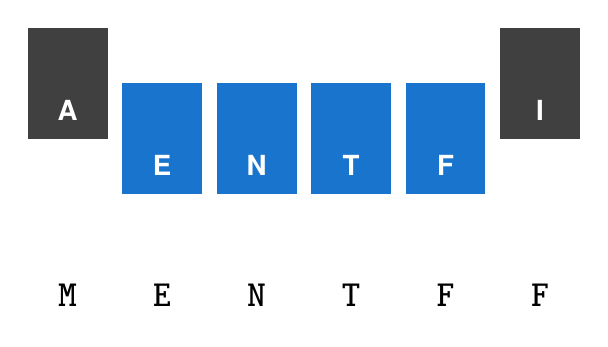
\begin{tikzpicture}
\colorlet{bgcol}{gray!15!white}
\tikzstyle{tcr}=[anchor=south,text=white,font=\bfseries];
\tikzstyle{eps}=[scale=1.3, anchor=south,text=black,font=\ttfamily];


\begin{scope}
      \foreach \x in {3.2,4.4,5.6,6.8}
        \filldraw[hivc] (\x,-0.1) rectangle +(1,1.4);
      \foreach \x in {2,8}
        \filldraw[darkgray] (\x,0.6) rectangle +(1,1.4);

        
        \node[tcr] at (2.5,0.7) {A};
        \node[tcr] at (3.7,0) {E};
        \node[tcr] at (4.9,0) {N};
        \node[tcr] at (6.1,0) {T};
        \node[tcr] at (7.3,0) {F};
        \node[tcr] at (8.5,0.7) {I};
     

	\node[eps] at (2.5,-1.7) {M};
        \node[eps] at (3.7,-1.7) {E};
        \node[eps] at (4.9,-1.7) {N};
        \node[eps] at (6.1,-1.7) {T};
        \node[eps] at (7.3,-1.7) {F};
        \node[eps] at (8.5,-1.7) {F};


\end{scope}


\end{tikzpicture}


\end{document}

